% !TeX root = RJwrapper.tex
\title{Transcriptional changes in the reproductive axis of parenting pigeons}
\author{by Rayna M Harris \footnote{equal contribtion}, Suzanne H. Austin \footnote{equal contribtion, currently at the
  University of Oregon}, Andrew S. Lang, Victoria S. Farrar, April Booth, Tanner Feustel, Matthew D. MacManes, Rebecca M. Calisi \footnote{corresponding author}}

\maketitle

\abstract{%
In species that provide parental care, successful rearing of offspring
involves a shift from aggressive and sexual behaviors to more caring and
nurturing ones. We hypothesize that these shifts in behavior are related
to changes in gene expression that are controlled by internal mechanisms
rather than by the external cues. We found that gene expression in the
hypothalamus is fairly insensitive to the natural transition between egg
and nestling stages; however, in the pituitary and gonads, gene
expression showed much more plasticity over the course of reproduction.
We show evidence that natural transitions in reproductive and parental
behavior by mediated internal clock controlling gene expression in the
pitary and gonads but that the hypothalamus is very sensitive to
external cues that signal a distruption in the natural parental care
cycle. This research provides a deeper understanding of the interplay of
genes, hormones, and parental care and has important implications for
understanding molecular processes that underlie behavior transitions.
}


\hypertarget{introduction}{%
\subsection{Introduction}\label{introduction}}

Reproduction is a critical period in an organism's life cycle. Parents
must balance their own needs with the energetic costs and
time-constraints required to successfully reproduce and rear their
offspring to independence (cite). A complex series of evolutionarily
conserved physiological processes underlie behaviors typically
associated with reproduction in vertebrates, including courtship,
nesting, and parental care. These processes are primarily mediated by
the reproductive axis, which consists of the hypothalamus in the brain,
the pituitary, and the gonads (i.e., the HPG). Our understanding of the
physiological changes that adults navigate as they transition through
reproductive states are primarily limited to a number of circulating
hormones and a small set of well-known genes (cite). We have yet to come
close to conceptualizing the larger symphony of reproductive events that
occur to yield reproductive and parental care behaviors.

Using the model of a biparental vertebrate species, the rock dove
(Columba livia), our team has previously demonstrated the dynamic nature
of gene activity within the reproductive or HPG axis.
\citet{MacManes2017} reported that HPG gene activity varied by sex, with
females exhibiting higher levels of overall gene expression than males.
\citet{Calisi2018} reported that HPG gene activity varied response to
restraint-stress, and Austin et al.~identify genes that responds to both
corticosterone treatment and restraint stress. While each of these
studies advanced our understanding of sex-differences and
transcriptional plasticity in the reproducitve axis, none of these
studies examined activity of the reproducitve axis of bird that are
actively reproducing or caring for offspring. Studying parental care in
both sexes of mammalian species is challenging because only the females
are able to use lactation to feed their young, and the physiological
mechanisms regulating this process are hard to control for. The rock
dove is an excellent system for studying reproduction and parental care
in both sexes because both males and females feed their young an
energy-rich secretion produced from the epithelial lining of their
crops, known as crop milk.

In this study, we investigate the activity of the HPG axis over the
course of reproduction and parental care by characterizing gene
expression as birds transition from non-breeding to nest-building, as
they lay and incubate their clutches, and finally as they become parents
and raise their chicks. Then, we conducted a series of nest
manipulations to ascertain constraints associated with biological timing
versus input from external stimuli. We conducted a comprehensive series
of analyses examine broad patterns of variation as well as the activity
of specific genes in specific tissues. We have also made our data and
scripts available so that others can reuse the data to ask different
questions or reproduce our results. This research provides a deeper
understanding of the interplay of genes, hormones, and parental care and
has important implications for understanding molecular processes that
underlie behavioral transitions. \citep[reviewed in][]{Lea1989} say
this, but other say that \citep[reviewed in][]{Dulac2014}.

\hypertarget{results}{%
\subsection{Results}\label{results}}

\emph{Data-driven characterization of reproductive and parental stage
groups.}

We first examined broad patterns of variation in gene expression in the
hypothalamus, pituitary, and gonads of male and female rock doves across
a series of timepoints that encapsulate important transitions in
reproduction and and parental care (Fig. 1A). t-Distributed Stochastic
Neighbor Embedding (t-SNE) is a nonlinear, dimension reduction technique
is used to visualize high-dimensional data (van der Maaten and Hinton
2008) and is widely used in in RNA sequencing to identify related and
distinct cell types (refs). Differential expespression profiling is
useful for pair-wise comparisons of differentially expressed genes
(DEGs) with positive log fold change (+LFC) in one group compared to
another. Combined, the provide stronger support for similarities and
differences between cell-types and treatment groups in multi-dimential
datasets. First, the data supports that the hypothalamus, pituitary, and
gonads have distinct gene expression profiles as evidenced by little
overlap in t-SNE space and an average of 13,000 DEGs between each tissue
(Fig. 1B). Second, the data supports that sex-differences are much more
promient in the gonads than in the brain (13,000 versus 2,000 DEGs)
(Fig. 1C). Because of these widespread tissue and sex-differences,
further ananlyses were conducted separately for each tissue and sex
(Fig. 1D, Suppl. Fig 1). In all the tissues, the control samples are
quiet different from all the other timepoints samples, and only a
fraction of the transcriptome is altered during the course of parental
care at the timepoints sampled. The most notable differences male and
female hpothalamic control samples are very different from on the rest
(\textasciitilde{}7000 DEGs, and only the two nestling care stages (n5
and n9)) show differential expression of more than 1,000 genes. In the
pituitary, late inubcation and hatch are quite simlilar to each other
and distinct from the earlier incubation stages stages, and temporal
changes in gene expression appears to be less variable in males than
females. In the female gonads there appear to be more changes in gene
expression early one, between nest building and early incuation, but the
male gonads show very little variation associated with parental stage.

\emph{Hypothesis-driven analysis of candidate parental-care genes.}

\begin{itemize}
\tightlist
\item
  Champagne Curley Genes (Fig 2)
\item
  GO genes (Fig 2 Suppl Fig 1)
\item
  Cancer genes (Fig 2 Suppl Fig 2)
\item
  Shiny genes (Fig 2 Suppl Fig 3)
\end{itemize}

\emph{Software for data exploration and hypothesis testing}

Data accessibility and reproducibility are key challenges for today's
researchers. Using Binder and Shiny, we have provides a means for
scientists, physicians, and the general public to explore the data,
code, and results from this project at
\url{https://raynamharris.shinyapps.io/musicalgenes/}. Like Hipposeq
(Cembrowski et al elife 2016, 2018), this tools allows quick and easy
data exploration of RNAseq data from mutiple cell types that relate to
brain function.

\hypertarget{discussion}{%
\subsection{Discussion}\label{discussion}}

This RNA-sequencing project was designed to characterize the
reproductive axis of bi-parental pigeons across a characteristic
reproductive cycle and through the parental main parental stages of egg
incubation and parental care using data- and hypotheses driven
approaches. We hypothesized that differences in gene expression would be
driven by either internal physiology or external stimuli. In the
pituitary, we found that the most explanatory source of variation in
gene expression was the expression level of prolactin (PRL). Circulating
levels of prolactin in the blood in this species are known to rise
around day nine and peak on or the day before hatch. Our results confirm
this and also identified one hundred genes whose expression is highly
correlated with prolactin. Today, this variation, which changes more
within a parental stage (e.g.~egg incubation or nestling care) suggests
that internal physiology drives changes in gene expression that precede
changes in external stimuli that lead to behavioral changes (e.g.~crop
milk or regurgitation). We predicted that either sex steroid peptide
hormones would play a role in governing the reproductive transitions,
but we did not anticipate discovering a link between PRL expression to
genes that are involved with DNA repair and regulation of the cycle.
Finally, we aimed to make these data and analyses FAIR (findable,
accessible, interoperable, and reproducible), open and reproducible to
encourage others to reuse our data to test new hypotheses or explore the
data with a different perspective or toolset. The scripts that made the
figures and tables are browseable online thanks to RStudio, GitHub and
Binder. The data can be visualized and sonified (turned into sound)
interactively thanks to RStudio, GitHub, and Shiny.

\hypertarget{materials-and-methods}{%
\subsection{Materials and Methods}\label{materials-and-methods}}

\emph{Animal Care}

All animal care and use comply with the Public Health Service Policy on
Humane Care and Use of Laboratory Animals and were approved by the
University of California, Davis IACUC permit \#18895. Birds were housed
at the University of California, Davis in enclosed aviaries with
\textasciitilde{}8 sexually reproductive adult pairs per aviary. All
adults birds are uniquely associated with nests by their unique color
band combination. Food and water were provided ad libitum, and nests
were monitored daily.

\emph{Experimental design and tissue processing}

To characterize reproduction and parental care, birds were sampled at 8
timepoints across the parental care cycle (Fig. 1a) as perviously
described in Austin et al 2020. Briefly, nest-building pairs where at
least was individual was seen carrying nesting material or shaping a
nest (bldg); the day the 1st egg was laid (lay), clutch completion (also
known as incubation day 3 (inc.d3)), mid-incubation (inc.d9), late
incubation (inc.d17), the day the first chick hatched (where hatch),
nestling care days 5 and 9 (n5 and n9). Additionally, a non-breeding
(control) timepoint was adding using control birds from previously
published studies (2,3).

To test our hypothesis that gene expression is govern more by internal
mechanisms than external cues, we conducted multiple offpsring
replacement or removal manipuations\ldots{}. Add details here.

To control for circadian rhythm confounds, each member of the pair was
collected between 0900-1200 (PST). We sampled a total of 331 birds (16
treatments with \textasciitilde{}10 pairs per treatment). Pairs were
captured and collected simultaneously within 5 min of entering their
cage, were anesthetized using isoflurane until unresponsive
(\textless{}2 min), and then decapitated. Trunk blood, brains,
pituitaries, and gonads were collected. Processing and analysis of truck
blood is described in Austin et al.~2020.

\emph{RNA sequencing analysis}

Processing of brains, pituitaries, and gonads for RNA sequenceing is
described in detail in Lang et al.~2020. Briefly, RNA from the
hypothalamus, pituitary, and gonads was processed for Illumina
sequencing using the NEB Next Ultra Directional RNA Library Prep Kit.
Reads were pseudomapped (insert Kalisto citation) to the Rock Dove
transcriptome v1.1.0 whose transcripts were annotated with genes from
Gallus gallus genome v5.

Statistical analyses and modeling were perforeming using R
\citep{RDevelopmentCoreTeam2013, Wickham2016}. Limma was use to process
all samples using the model \textasciitilde{} tissue * sex * treatment
(citation). t-Distributed Stochastic Neighbor Embedding (t-SNE) analysis
was conducted using a perplexity of 10 \citep{VanDerMaaten2008}.
Principal Component Analysis (PCA) was conducted using the top 500 most
varying genes (citation). DESeq2 was used to model gene express for sex
and tissue combination separately using the model
\textasciitilde{}treatment \textbackslash{}citep\{Love2014). Weighted
correlation network analysis (WGCNA) was used to identify set of genes
with simliar patterns of gene expression over the course of reprodution
and parental care (citation). ANOVAs were used to test whether specific
genes were differnetially expressed between between sequential
timepoints.

\emph{Data availablility}

RNA sequencing data for available through the European Nucleotide
Archive (ENA) project ID PRJEB16136 and XXXXX. Code and data for
reproducing the results described in the manuscript are available at
\url{https://github.com/macmanes-lab/DoveParentsRNAseq} (upload to zendo
and cite). Data can be explored in the cloud using Binder
\citep{project_jupyter-proc-scipy-2018}.

\hypertarget{acknowledgements}{%
\subsection{Acknowledgements}\label{acknowledgements}}

Thanks to Owen for discussion of data sonfification. Thanks to DIB lab
members for software and methods discussion (Titus, Taylor, Luiz,
Amanda, Alicia, Picaso). We thank Pacha for help with database and
Shiny.

We thank Irene, Erica, Beth Krestoff and Tiffany Chen for assistance in
managing the aviary and collecting nest stage data. We thank Candice
Lee, Annie Bond, and Tanner Feustel and others?? for assistance with
tissue collections. We thank Dr.~Fred Angelier for performing the
prolactin RIA.This research was supported by NSF IOS 1455960 to R.M.C.
and M.D.M. Author contributions: RMC designed the experiment. RMC and
MDM acquired funding. SHA contributed to the experimental design by
adding several time points. SHA, with the assistance of VF, AB, and RMC,
conducted the data collection. SHA and a team of trained undergraduate
students biopsy punched the hypothalami and lateral septum. ASL
extracted the RNA, created the libraries, and conducted all early
bioinformatic work. RMH conducted all later analyses of the genomic
data. RMH and SHA drafted the manuscript and all other authors provided
edits.

\hypertarget{references}{%
\subsection{References}\label{references}}

\bibliography{RJreferences}

\newpage

\textbackslash{}begin\{figure\}{[}h{]} \centering
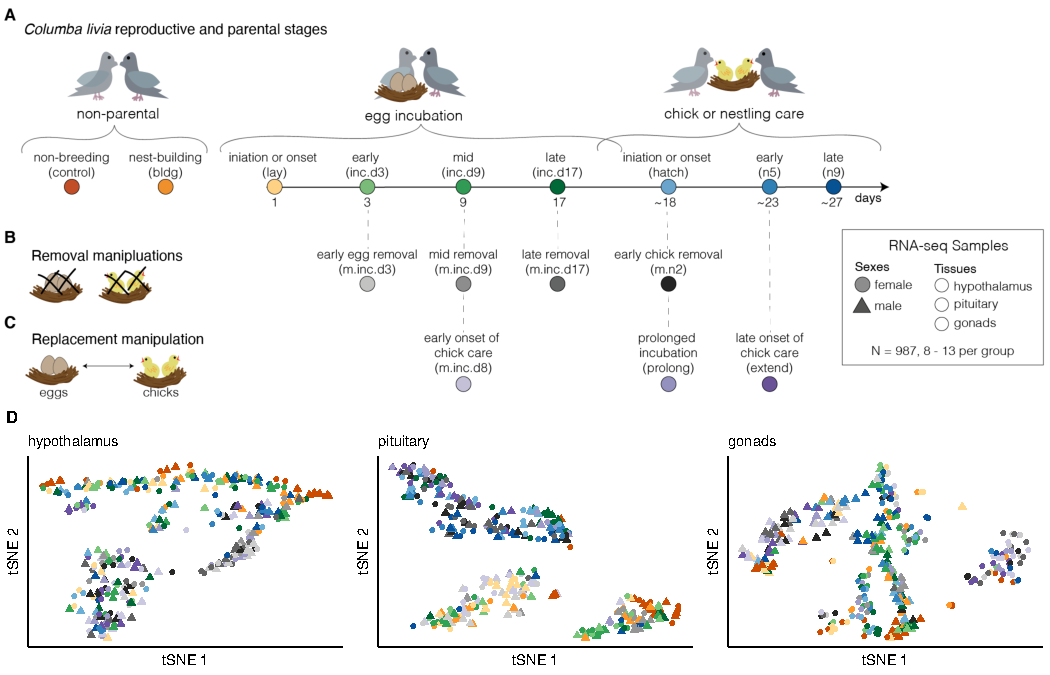
\includegraphics[width=1.0\textwidth]{../../figures/fig1-1}
\textbackslash{}caption\{Broad patterns of variation in hypothalamic,
pituitary, and gonadal gene expression in male and female rock doves
across reproductive and parental transitions.** A) Experimental design.
B) The t-SNE plot shows all 636 samples as points in space colored by
tissue with ellipses drawn around show 95\% confidence interval, and the
bar plots show the total number of differentially expressioned genes
(DEGs) whose expression was significantly higher in one tissue versus
the other. C) This t-SNE plot shows the same data points colored by sex
while the ellipses delinate the source tissue; bar plots show the DEGs
between the sexes for each tissue. D) These t-SNE and bar plots provide
insight into the temporal differences in gene expression within each
tissue for each sex. Here, the bar plots highlight the number of DEGs
between each sequential time point. For comparisons to controls, see
fupplemental figure 1.\} \label{figure:fig1}
\textbackslash{}end\{figure\}

\begin{figure}[h]
  \centering
  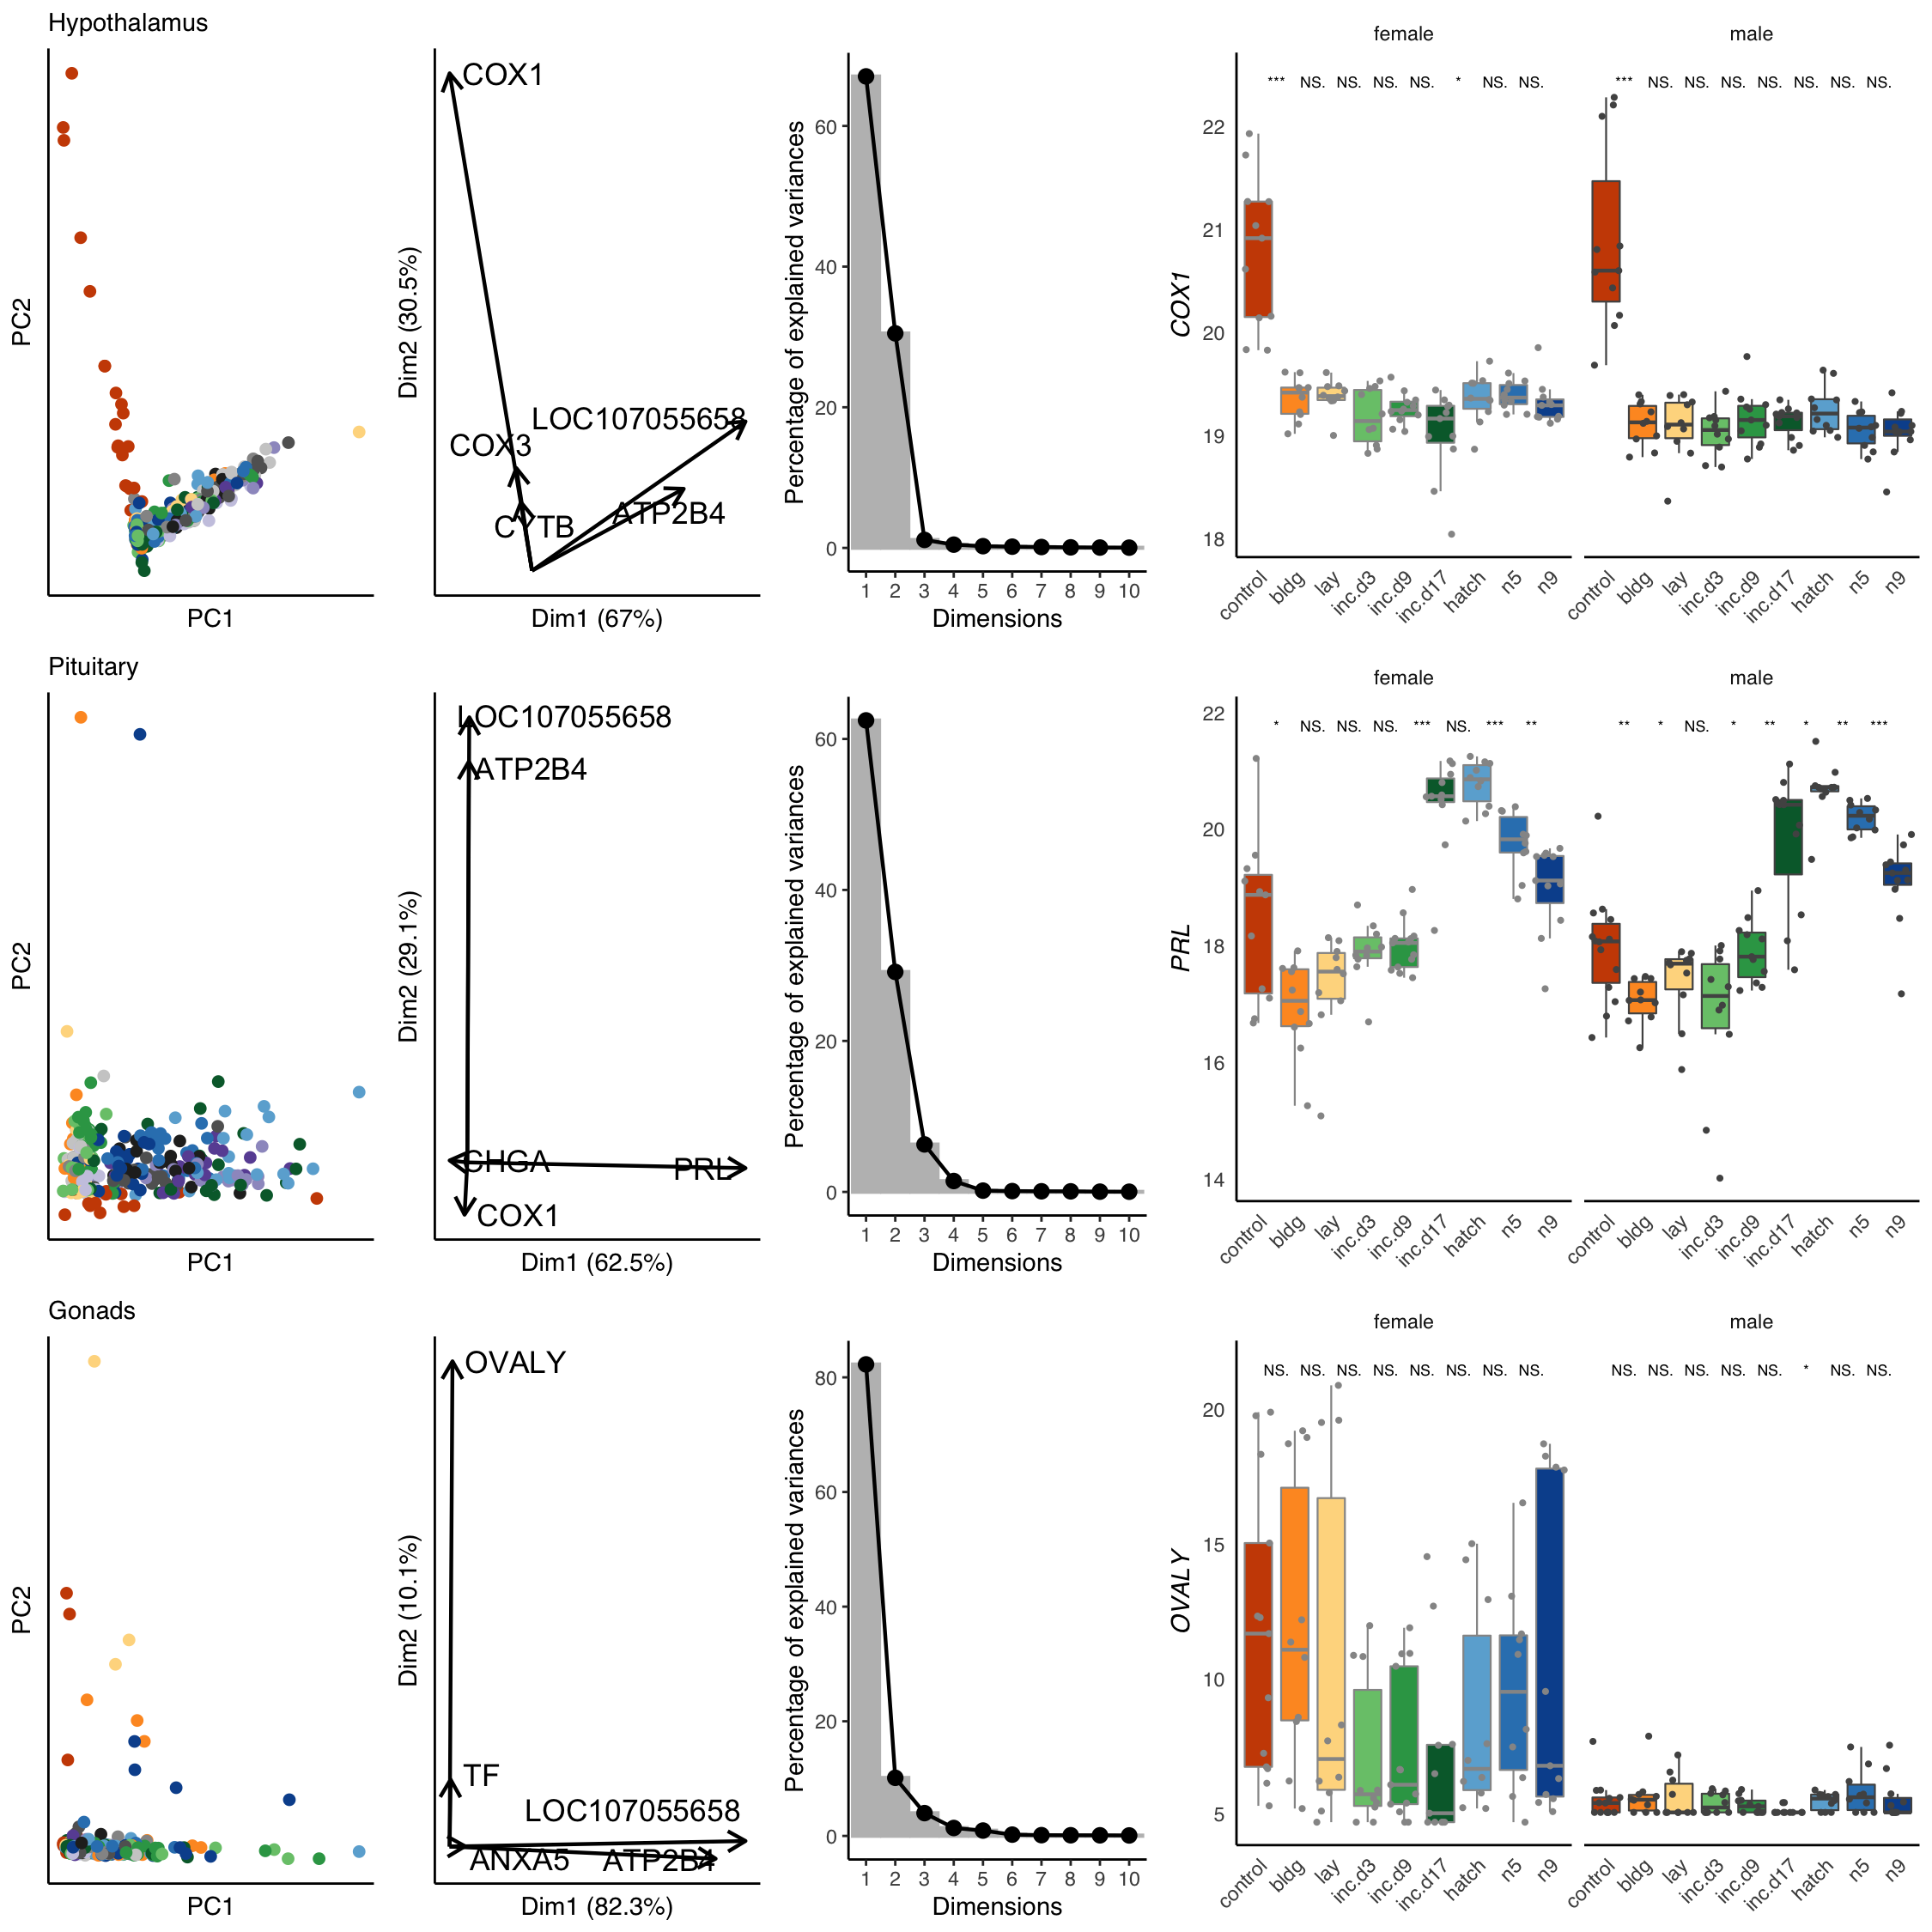
\includegraphics[width=1.0\textwidth]{../../figures/supplfig-1-1}
  \caption{Summary of the total number of differentially expressed genes (DEGs) from pair-wise comparison using DESeq2.** Bar plots showing the total number of differentially expressed genes (p < 0.1) and colored by the direction of increased expression (or positive log fold change (+LFC))  are shown for three different analysis: relative to the control group (A), the nest-building (bldg) group (B), and the previous sampling timepoint (C).}
  \label{figure:supplfig1}
\end{figure}

\newpage

\begin{figure}[h]
  \centering
  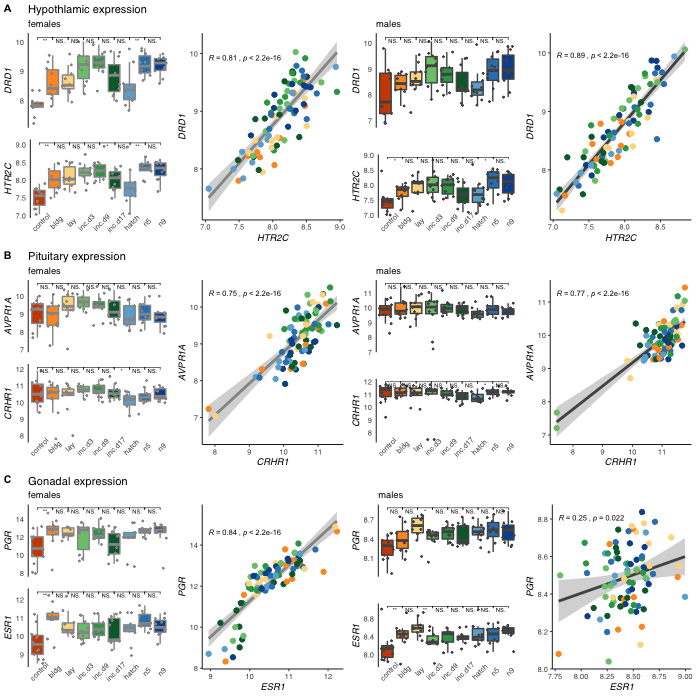
\includegraphics[width=1.0\textwidth]{../../figures/fig2-1}
  \caption{Differential gene expression differences between sequential parental stages. a) We calculated the differentail gene expression between each consequtive parental stage samples, for a total of 8 pair-wise comparisons for each sex in each tissue. The y-axis of these bar plots displays the total number of differentially expressed genes for each comparsison in the hypothalamus (b), pituitary (c), gonads (d). Bars are collored by the direction of the change in gene expression. Control: control: red or , nest-building (bldg): orange, lay: yellow; incubation day 3 (inc.d3): light green, inc.d9: green, inc.d17: dark green, hatch: dark blue, nestling care day 5 (n5): blue, and n9: light blue.}
  \label{figure:fig2}
\end{figure}

\newpage

\begin{figure}[ht]
  \centering
  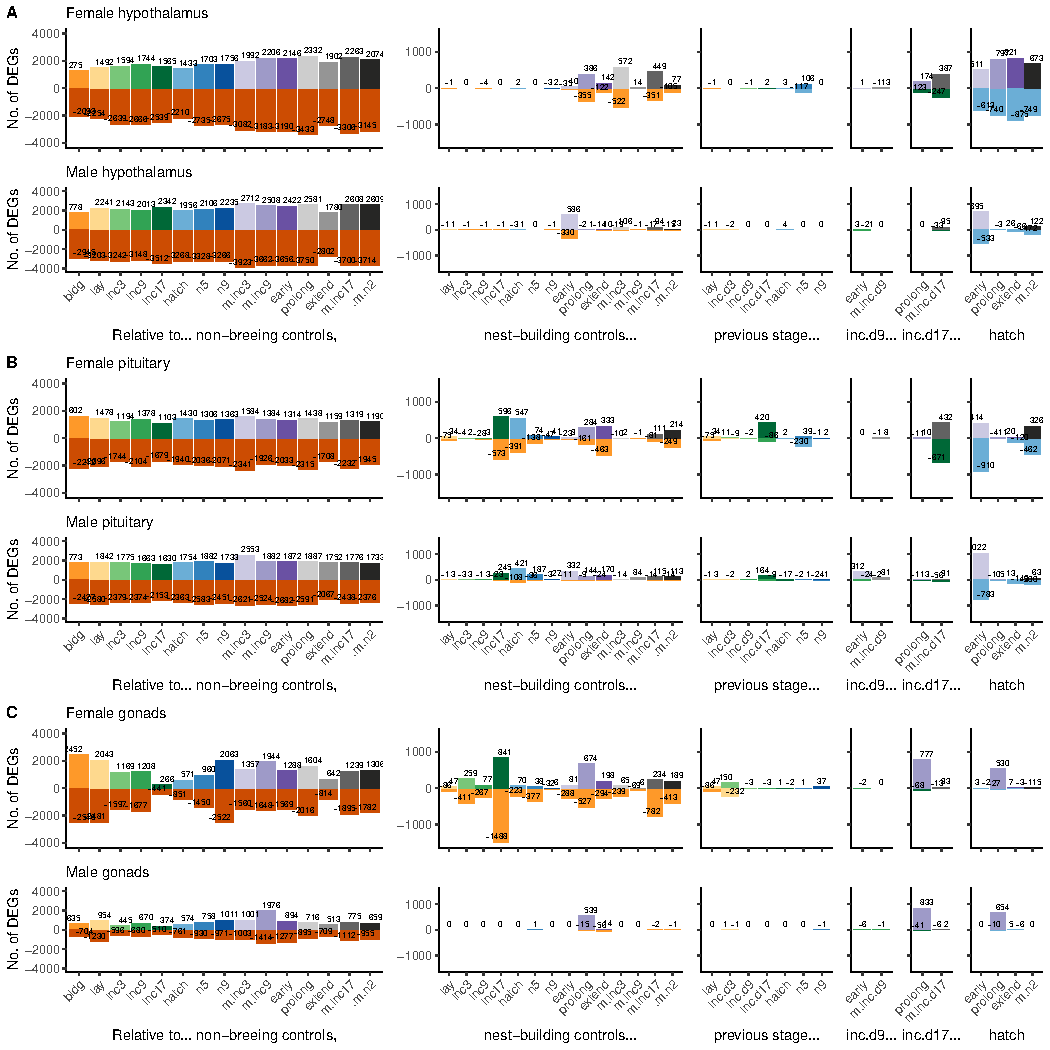
\includegraphics[width=1.0\textwidth]{../../figures/fig3-1}
  \caption{Another another figure}
  \label{figure:fig3}
\end{figure}

\newpage

\begin{figure}[ht]
  \centering
  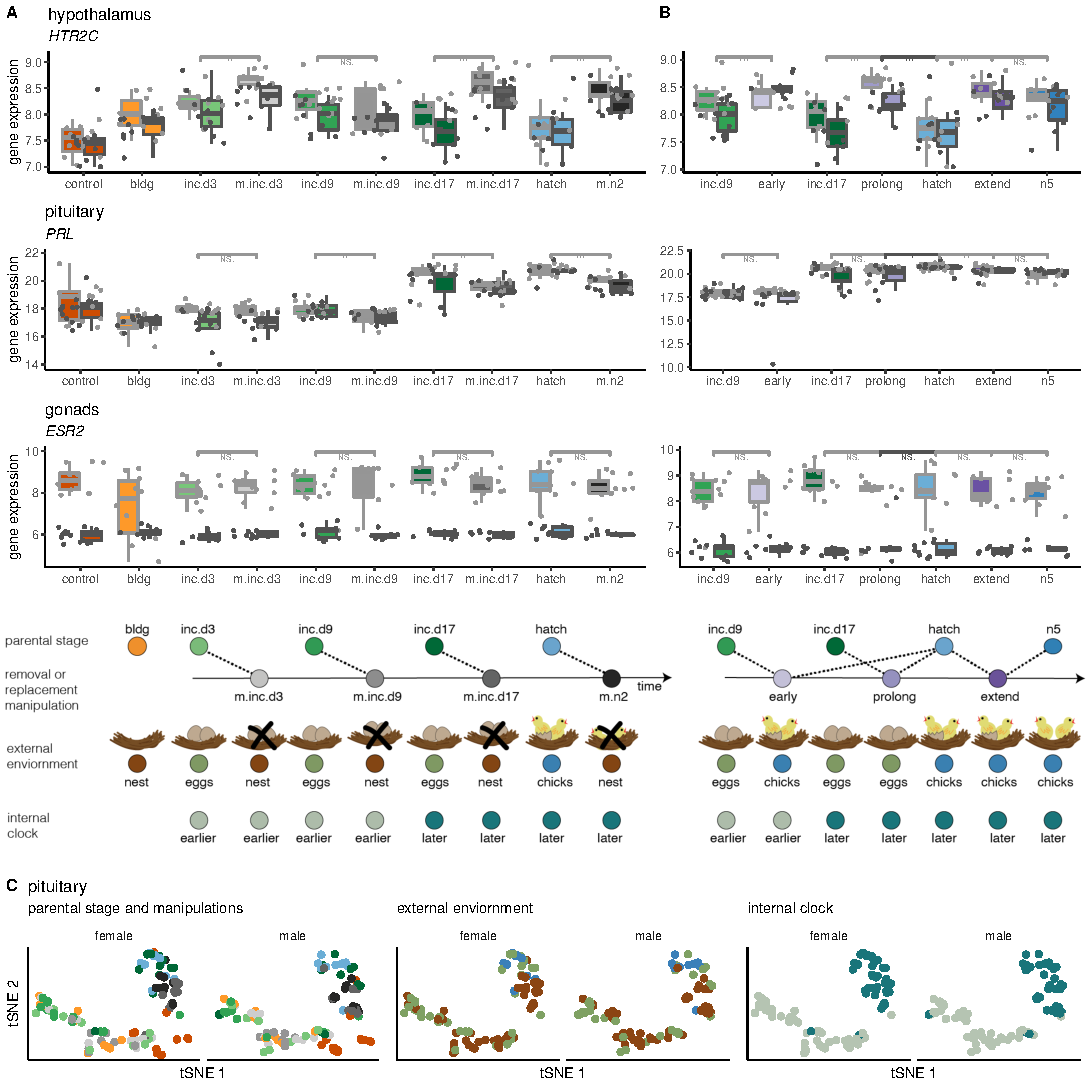
\includegraphics[width=1.0\textwidth]{../../figures/fig4-1}
  \caption{Another another figure}
  \label{figure:fig4}
\end{figure}

\newpage

\newpage

\hypertarget{author-affiliations}{%
\subsection{Author affiliations}\label{author-affiliations}}


\address{%
Rayna M Harris \footnote{equal contribtion}\\
University of California, Davis\\
\\
}


\address{%
Suzanne H. Austin \footnote{equal contribtion, currently at the
  University of Oregon}\\
University of California, Davis\\
\\
}


\address{%
Andrew S. Lang\\
University of New Hampshire\\
\\
}


\address{%
Victoria S. Farrar\\
University of California, Davis\\
\\
}


\address{%
April Booth\\
University of California, Davis\\
\\
}


\address{%
Tanner Feustel\\
University of California, Davis\\
\\
}


\address{%
Matthew D. MacManes\\
University of New Hampshire\\
\\
}


\address{%
Rebecca M. Calisi \footnote{corresponding author}\\
University of California, Davis\\
\\
}
\href{mailto:rmcalisi@ucdavis.edu}{\nolinkurl{rmcalisi@ucdavis.edu}}

